
\documentclass[a4paper,12pt]{article}
\usepackage[utf8]{inputenc}
\usepackage[a4paper,
            bindingoffset=0.2in,
            left=1in,
            right=1in,
            top=1in,
            bottom=1in,
            footskip=.25in]{geometry}


%###############################################################################

%\input{~/layout/global_layout}


%###############################################################################

% packages begin

\usepackage[
  backend=biber,
  sortcites=true,
  style=alphabetic,
  eprint=true,
  backref=true
]{biblatex}
\addbibresource{bibliography.bib}

\usepackage{euscript}[mathcal]
% e.g. \mathcal{A} for fancy letters in mathmode
\usepackage{amsmath,amssymb,amstext,amsthm}

\usepackage{mdframed}
\newmdtheoremenv[nobreak=true]{problem}{Problem}[subsection]
\newmdtheoremenv[nobreak=true]{claim}{Claim}[subsection]
\newtheorem{definition}{Definition}[subsection]
\newtheorem{lemma}{Lemma}[claim]
\newtheorem{plemma}{Lemma}[problem]

\usepackage{mathtools}
\DeclarePairedDelimiter\ceil{\lceil}{\rceil}
\DeclarePairedDelimiter\floor{\lfloor}{\rfloor}

\usepackage{enumerate}
\usepackage[pdftex]{graphicx}
\usepackage{subcaption}
% 'draft' für schnelleres rendern mitübergeben -> [pdftex, draft]
% dadruch wird nicht das bild mitgerendered, sondern nur ein kasten mit bildname -> schont ressourcen

\usepackage{hyperref}

\usepackage{tikz}
\usetikzlibrary{arrows,automata,matrix,positioning,shapes}

% for adding non-formatted text to include source-code
\usepackage{listings}
\lstset{language=Python,basicstyle=\footnotesize}
% z.B.:
% \lstinputlisting{source_filename.py}
% \lstinputlisting[lanugage=Python, firstline=37, lastline=45]{source_filename.py}
%
% oder
%
% \begin{lstlisting}[frame=single]
% CODE HERE
%\end{lstlisting}
\usepackage{algorithm}
\usepackage{algpseudocode}

\usepackage{wasysym}

\usepackage{titling}
\usepackage{titlesec}
\usepackage[nocheck]{fancyhdr}
\usepackage{lastpage}

\usepackage{kantlipsum}
\usepackage[colorinlistoftodos,prependcaption,textsize=tiny]{todonotes}

% packages end
%###############################################################################

\pretitle{% add some rules
  \begin{center}
    \LARGE\bfseries
} %, make the fonts bigger, make the title (only) bold
\posttitle{%
  \end{center}%
  %\vskip .75em plus .25em minus .25em% increase the vertical spacing a bit, make this particular glue stretchier
}
\predate{%
  \begin{center}
    \normalsize
}
\postdate{%
  \end{center}%
}

\titleformat*{\section}{\Large\bfseries}
\titleformat*{\subsection}{\large\bfseries}
\titleformat*{\subsubsection}{\normalsize\bfseries}

\titleformat*{\paragraph}{\Large\bfseries}
\titleformat*{\subparagraph}{\large\bfseries}

%###############################################################################
% TODO define Headers and Fotter

\pagestyle{fancy}
\fancyhf{}
% l=left, c=center, r=right; e=even_pagenumber, o=odd_pagenumber; h=header, f=footer
% example: [lh] -> left header, [lof,ref] -> fotter left when odd, right when even
%\fancyhf[lh]{}
%\fancyhf[ch]{}
%\fancyhf[rh]{}
%\fancyhf[lf]{}
\fancyhf[cf]{\footnotesize Page \thepage\ of \pageref*{LastPage}}
%\fancyhf[rf]{}
\renewcommand{\headrule}{} % removes horizontal header line

% Fotter options for first page

\fancypagestyle{firstpagestyle}{
  \renewcommand{\thedate}{\textmd{}} % removes horizontal header line
  \fancyhf{}
  \fancyhf[lh]{\ttfamily M.Sc. Computer Science\\KTH Royal Institute of Technology}
  \fancyhf[rh]{\ttfamily Period 3\\\today}
  \fancyfoot[C]{\footnotesize Page \thepage\ of \pageref*{LastPage}}
  \renewcommand{\headrule}{} % removes horizontal header line
}
%###############################################################################
% Todo: define Title

\title{
  \normalsize{DD2358 VT25 Introduction to}\\
  \normalsize{High Performance Computing}\\
  \large{Assignment 2}\\
}
\author{
  \small Lennart Herud\\[-0.75ex]
%  \footnotesize\texttt{MN: }\\[-1ex]
  \scriptsize\texttt{herud@kth.se}
  \and
    \small Paul Mayer\\[-0.75ex]
%  \footnotesize\texttt{MN: }\\[-1ex]
  \scriptsize\texttt{pmayer@kth.se}
  \and
    \small Adrian Sušec\\[-0.75ex]
%  \footnotesize\texttt{MN: }\\[-1ex]
  \scriptsize\texttt{susec@kth.se}
  \and
  \small Rishi Vijayvargiya\\[-0.75ex]
%  \footnotesize\texttt{MN: }\\[-1ex]
  \scriptsize\texttt{rishiv@kth.se}
}
\date{}

%###############################################################################
% define Commands

\newcommand{\N}{\mathbb{N}}
\newcommand{\R}{\mathbb{R}}
\newcommand{\Z}{\mathbb{Z}}
\newcommand{\I}{\mathbb{I}}

\newcommand{\E}{\mathbb{E}}
\newcommand{\Prob}{\mathbb{P}}

\renewcommand{\epsilon}{\varepsilon}

% Todo: Set Counter to Excercise Sheet Number
%\setcounter{section}{1}
%\setcounter{subsection}{1}

%###############################################################################
%###############################################################################

\begin{document}
\maketitle
\thispagestyle{firstpagestyle}

% \tableofcontents
\listoftodos

\vspace{1em}

%---
%
\section*{Prefix}
\todo[inline]{Make sure title and headers are correctly changed!}
\todo[inline]{Change counter to match excercise sheet}

% content begin
%

\section{PyTest with the Julia Set Code}
\section{Python DGEMM Benchmark Operation}
\section{Experiment with the Python Debugger}
\section{Bonus: Game of Life}
For this task, we examined the code for \textit{Game of Life} found at this location: \url{https://github.com/electronut/pp/blob/master/conway/conway.py}. The working directory for our assignment code referenced in this section is the \verb|bonus/| directory found at this location: \url{https://github.com/paulmyr/DD2358-HPC25/tree/master/02_hpcds/bonus}. All the profiling, timing, and optimizations that follow were performed on a 2021 MacBook Pro with Apple's M1 Chip. More info on its specifications can be found \href{https://support.apple.com/en-us/111901}{here}.
\subsection{B.1: Linting and Documentation}
We ran \verb|pylint| on the default \verb|conway.py| file above, and got output that was mostly comprised of warnings/convention/refactor related information. To fix these issues, we used the \verb|black| auto-formatter on the default \verb|conway.py| file, and amended some of these issues (such as missing docstring for a function, or snake-case conformity) manually. Afterwards, only one issue was remaining in the default \verb|conway.py| file -- which had to do with the unused variable \verb|frame_num| for the function \verb|update|. This was left as is, since we believe this was used by the animation function of \verb|matplotlib| to visualize the grid. Information on the output of \verb|pylint| on the default \verb|conway.py| file can be found in the \verb|misc/linting_outputs.txt| file in the repository. 

To generate the documentation, we used the \verb|sphinx| tool on the \verb|conway.py| file after it was modified above to conform to as many python standards as possible (according to \verb|pylint|). The generated documentation can be accessed by clicking on the \verb|docs/html/index.html| page in the working directory for the bonus. Help of this useful tutorial on the \verb|sphinx| tool was taken to generate the documentation: \url{https://www.youtube.com/watch?v=BWIrhgCAae0} (including steps such as modifying the \verb|docs/source/conf.py| file, or generating the required \verb|reStructuredText| (ie, files with extension \verb|rst|) files. An example of clicking on the \verb|conway module| after opening the \verb|docs/html/index.html| page can be seen below

\begin{figure}[h!]
  \centering
  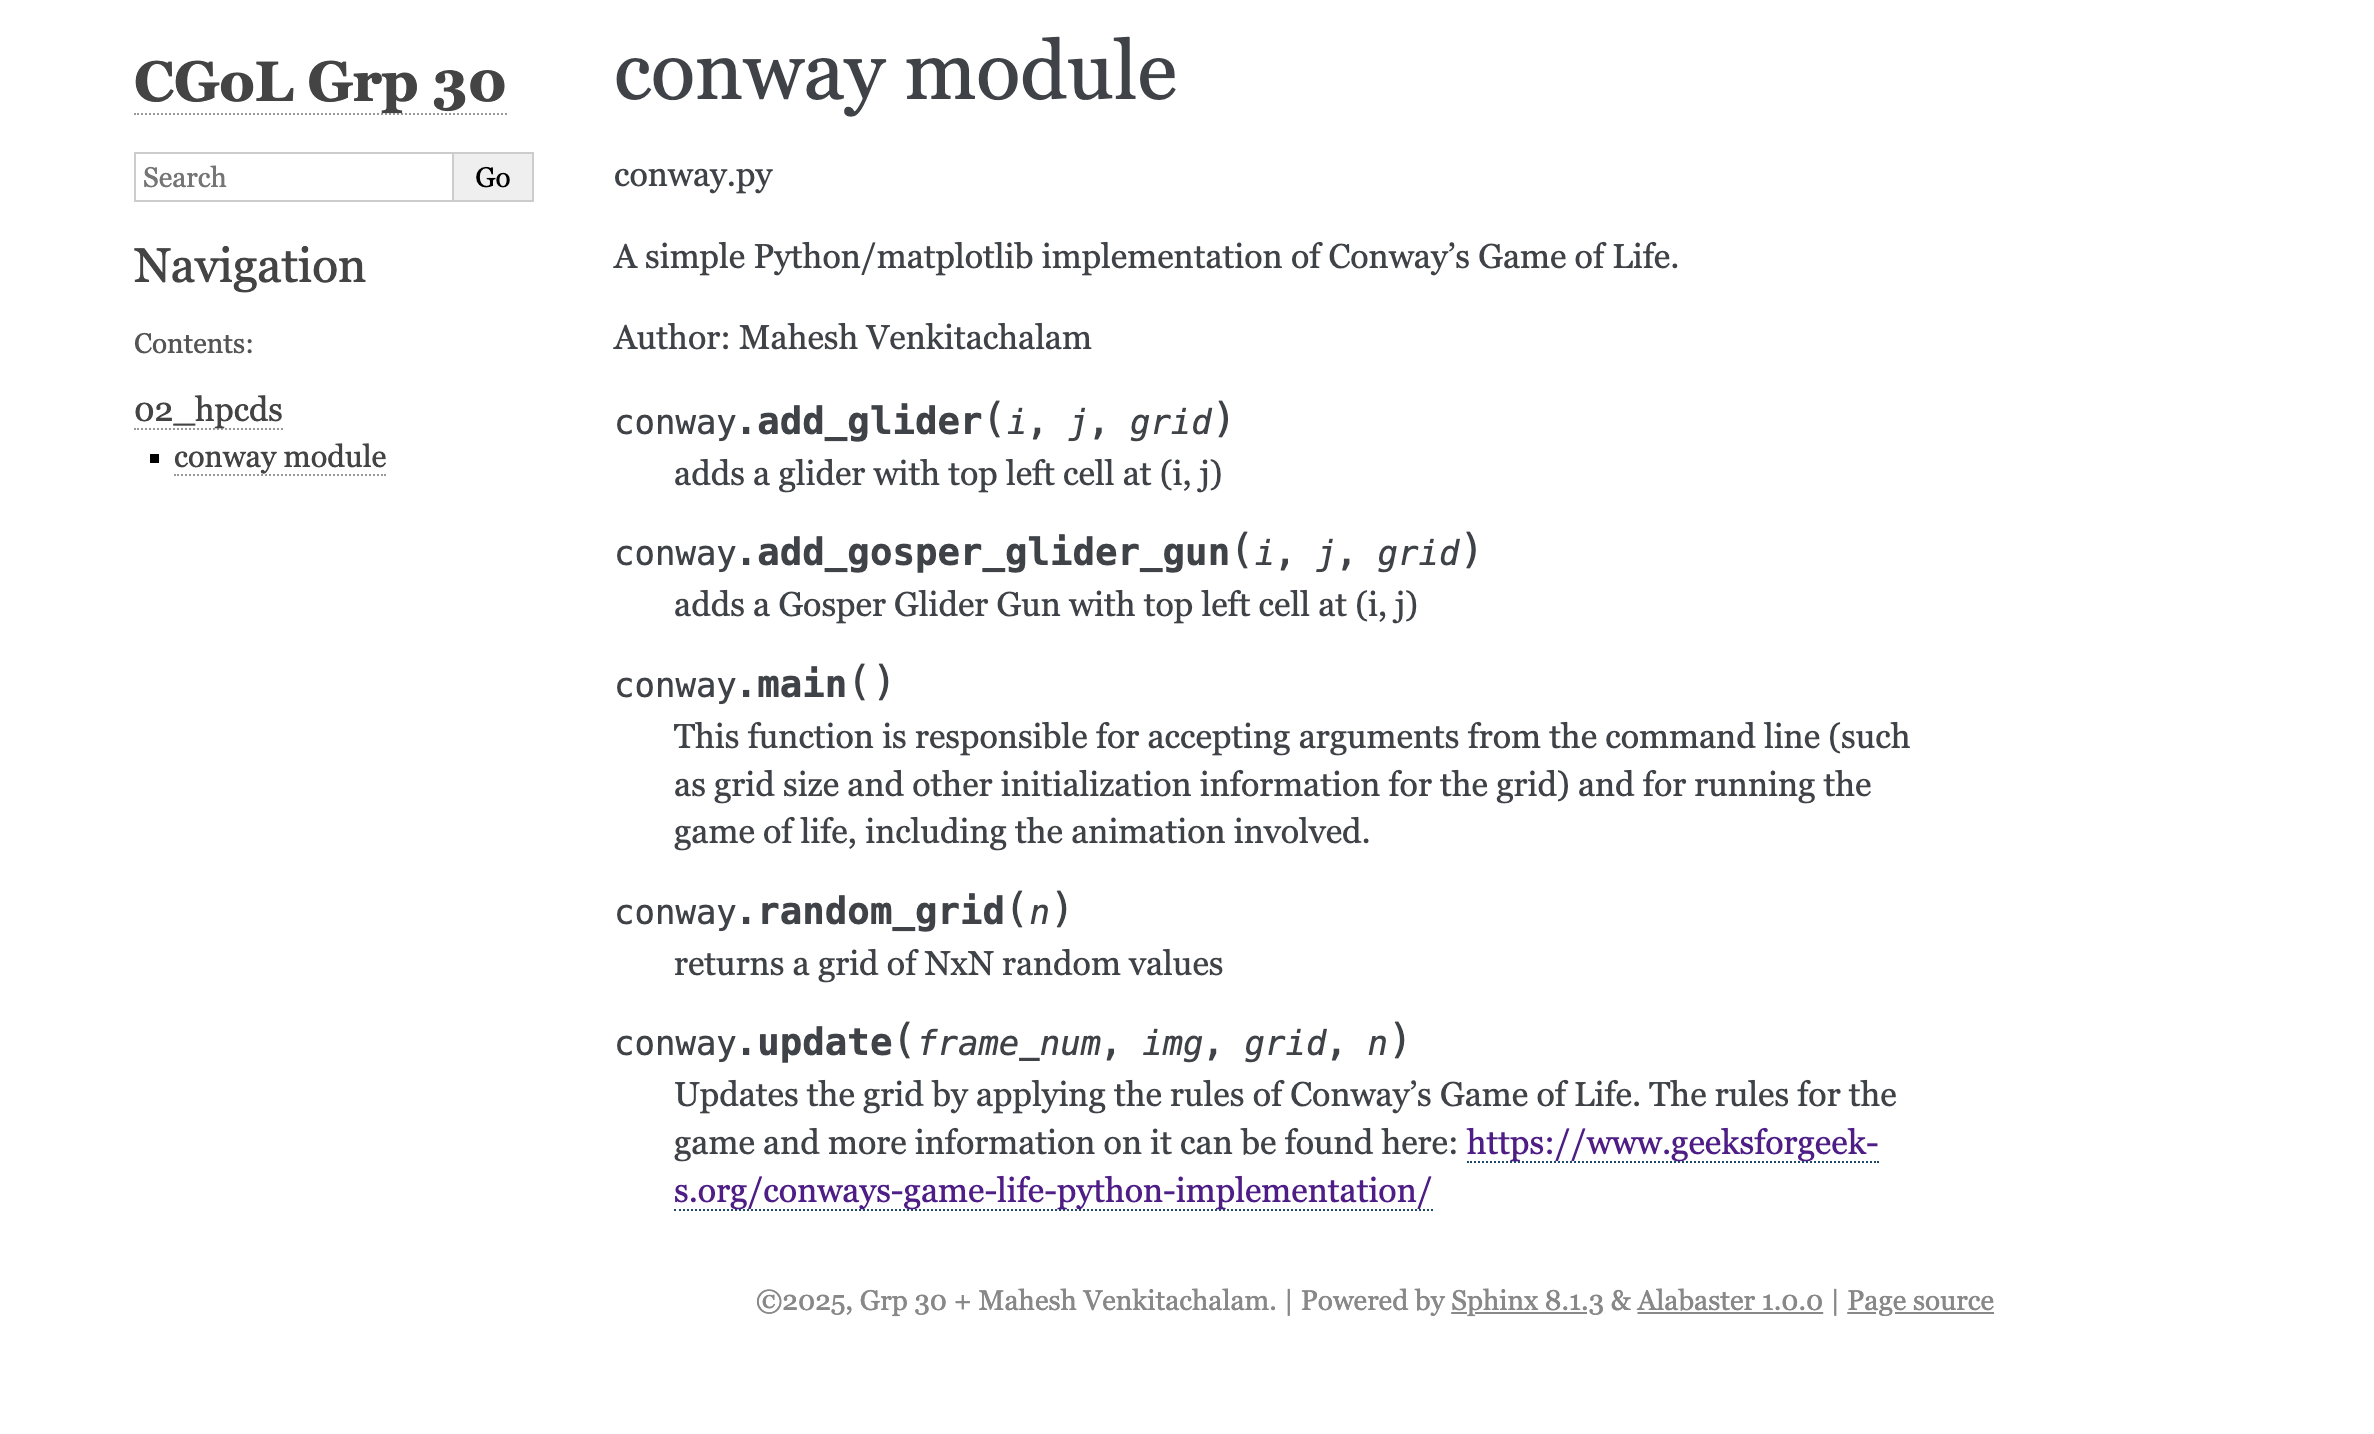
\includegraphics[width=\textwidth]{images/conway_documentation_example.png}
  \caption{Documentation for the Default conway.py File}
  \label{fig:conway_docs}
\end{figure}

Note that we only generated this documentation when only the default \verb|conway.py| file was present (as this was a part preceding the later steps of the Bonus exercise). Thus, only documentation on  the original \verb|conway.py| file (after fixing most of the linting issues) can be found on the docs generated by \verb|sphinx|. The same applies for running \verb|pylint| and \verb|black| -- these commands were only ran on the original \verb|conway.py| file (not any other files present in the repo or used in this bonus section).

\subsection{B.2: Execution Time and Plot}
To profile the code, we measured the execution time of the main function that is responsible for updating the state of the grid based on the rules of \textit{Game of Life} -- the \verb|update| function. the code that we used for profiling can be found in the \verb|conway_profile.py| file under the working directory (present \href{https://github.com/paulmyr/DD2358-HPC25/blob/master/02_hpcds/bonus/conway_profile.py}{here}). This code removes the code responsible for creating different specific patterns on the grid based on user arguments (along with the code to process user arguments), and the code to visualize the grid using \verb|matplotlib|. Thus, only the \verb|update| function and the function responsible for initializing the grid (with a seed of 42) are kept from the original \verb|conway.py| file. The \verb|profile_vanilla_computation| method is responsible for doing the profiling. We start at a $64 \times 64$ grid, incrementing by multiples of 2 until we reach a $1024 \times 1024$ grid. We count the average time of doing 50 updates to the starting grid (over 10 runs). 

To prevent repitition, the results of timing the original \verb|update| code (both textual data and the graph) will be presented along with the results of timing our optimized function (the \verb|update_vectorized| in the same file). This can be found under the \hyperref[sec:b4]{Optimization and Results} section.

\subsection{B.3: Profiling Existing Code}
\label{sec:b3}
We felt that the only function that was doing compute-heavy operations that would dictate the running time of the algorithm would be the \verb|update| function. Thus, we decided to use \verb|line_profiler| to profile the \verb|update| function. Inside this function, our hypothesis was that the operation to compute the \verb|total| for each grid celll would be the most computationally expensive operation. 

The profiling was done on the \verb|conway_profile.py| file -- which had the barebones implementation from \verb|conway.py| (without the special cases and visualizations, as described above). There, we decided to use \verb|line_profiler| on 2 functions -- the \textit{calling} function \verb|profile_vanilla_computation|, and the \textit{called} function \verb|update|. We performed only 1 run with 50 updates, on a grid of size $64 \times 64$. On doing so, we obtained the following results: 

\begin{lstlisting}[language=bash,basicstyle=\tiny\ttfamily]
$ python3 -m line_profiler -rmt "conway_profile.py.lprof"
Timer unit: 1e-06 s

Total time: 0.632629 s
File: conway_profile.py
Function: update at line 28

Line #      Hits         Time  Per Hit   % Time  Line Contents
==============================================================
    28                                           @profile                                                                                   
    29                                           def update(grid, n):                                                                       
   [...function docstring...]
    35                                               # copy grid since we require 8 neighbors for calculation                               
    36                                               # and we go line by line                                                               
    37        50        105.0      2.1      0.0      new_grid = grid.copy()                                                                 
    38      3250        339.0      0.1      0.1      for i in range(n):                                                                     
    39    208000      24151.0      0.1      3.8          for j in range(n):                                                                 
    40                                                       # compute 8-neghbor sum                                                        
    41                                                       # using toroidal boundary conditions - x and y wrap around                     
    42                                                       # so that the simulaton takes place on a toroidal surface.                     
    43    409600      42309.0      0.1      6.7              total = int(                                                                   
    44    204800      21815.0      0.1      3.4                  (                                                                          
    45   1638400     241913.0      0.1     38.2                      grid[i, (j - 1) % n]                                                   
    46    204800      30106.0      0.1      4.8                      + grid[i, (j + 1) % n]                                                 
    47    204800      32619.0      0.2      5.2                      + grid[(i - 1) % n, j]                                                 
    48    204800      30382.0      0.1      4.8                      + grid[(i + 1) % n, j]                                                 
    49    204800      32510.0      0.2      5.1                      + grid[(i - 1) % n, (j - 1) % n]                                       
    50    204800      31131.0      0.2      4.9                      + grid[(i - 1) % n, (j + 1) % n]                                       
    51    204800      32163.0      0.2      5.1                      + grid[(i + 1) % n, (j - 1) % n]                                       
    52    204800      32481.0      0.2      5.1                      + grid[(i + 1) % n, (j + 1) % n]                                       
    53                                                           )                                                                          
    54    204800      14930.0      0.1      2.4                  / 255                                                                      
    55                                                       )                                                                              
    56                                                       # apply Conway's rules                                                         
    57    204800      39194.0      0.2      6.2              if grid[i, j] == ON:                                                           
    58     30759       4151.0      0.1      0.7                  if (total < 2) or (total > 3):                                             
    59     13261       2062.0      0.2      0.3                      new_grid[i, j] = OFF                                                   
    60                                                       else:                                                                          
    61    174041      18131.0      0.1      2.9                  if total == 3:                                                             
    62     12867       2016.0      0.2      0.3                      new_grid[i, j] = ON                                                    
    63                                                                                                                                      
    64        50        121.0      2.4      0.0      grid[:] = new_grid[:]                                                                  


Total time: 1.42833 s
File: conway_profile.py
Function: profile_vanilla_computation at line 94

Line #      Hits         Time  Per Hit   % Time  Line Contents
==============================================================
    94                                           @profile                                                                                        
    95                                           def profile_vanilla_computation(update_method_key):                                             
    96                                               # grid sizes increase by powers of 2                                                        
    97                                               # grid_sizes = [64, 128, 256, 512, 1024]                                                    
    98         1          1.0      1.0      0.0      grid_sizes = [64]                                                                           
    99                                               # grid_sizes = [64, 128]                                                                    
   100                                               # times for each of the computations (in seconds)                                           
   101         1          0.0      0.0      0.0      times = []                                                                                  
   102                                               # number of iterations for which the updates will happen                                    
   103         1          0.0      0.0      0.0      max_iters = 50                                                                              
   104                                               # The number of times the run will be performed for each grid size.                         
   105                                               # The final running time reported will be the average of these runs                         
   106                                               # num_runs = 10                                                                             
   107         1          0.0      0.0      0.0      num_runs = 1                                                                                
   108                                                                                                                                           
   109         1         20.0     20.0      0.0      print(...actual print statement omitted for space...)
   110                                                                                                                                           
   111         2          2.0      1.0      0.0      for curr_size in grid_sizes:                                                                
   112         1          0.0      0.0      0.0          total_time = 0                                                                          
   113                                                                                                                                           
   114         2          0.0      0.0      0.0          for _ in range(num_runs):                                                               
   115         1        361.0    361.0      0.0              curr_grid = random_grid(curr_size)                                                  
   116                                                                                                                                           
   117         1          1.0      1.0      0.0              t1 = timer()                                                                        
   118        51          5.0      0.1      0.0              for _ in range(max_iters):                                                          
   119        50    1427921.0  28558.4    100.0                  UPDATE_DICT[update_method_key](curr_grid, curr_size)                            
   120         1          3.0      3.0      0.0              t2 = timer()                                                                        
   121                                                                                                                                           
   122         1          1.0      1.0      0.0              total_time += (t2 - t1)                                                             
   123                                                                                                                                           
   124         1          1.0      1.0      0.0          times.append(total_time / num_runs)                                                     
   125         1         17.0     17.0      0.0          print(...statement omitted for space...)                 
   126                                                                                                                                           
   127         1          1.0      1.0      0.0      return (grid_sizes, times)                                                                  


  0.63 seconds - conway_profile.py:28 - update
  1.43 seconds - conway_profile.py:94 - profile_vanilla_computation
\end{lstlisting}
It is clearly evident that in the \verb|profile_vanilla_computation| function, almost all the time is spent calling the \verb|update| function (the use of an \verb|UPDATE_DICT| was done for ease-of-use when using this file with the vectorized update as well, but here it just calls the sub-optimal \verb|update| function). Inside the \verb|update| function, it is also evident that most of the time (upto $38\%$) seems to be spent inside the nested for-loops: computing the value of \verb|total| and the \verb|ON, OFF| state of the \verb|new_grid|. 
This confirms our hypothesis that the nested-loops are the main bottleneck of the current implementation, and thus effort should be spent optimzing these updates. \\
\textit{Note: We did not have access to the perf tool, since this was performed on a Macbook}.

\subsection{B.4: Optimization and Results}
\label{sec:b4}
The optimization we implemented vectorized the computations being done in the nested for-loops of the sub-optimal \verb|update| function with the help of the \verb|numpy| library. This optimization took inspiration from the the optimization of the Diffusion Process presented during lectures, and the optimization of \textit{Game of Life} presented in \href{https://www.labri.fr/perso/nrougier/from-python-to-numpy/}{this} guide by Nicolas Rougier. The optimized implementation can be found in the \verb|update_vectorized| method of the \verb|conway_profile.py| file \href{https://github.com/paulmyr/DD2358-HPC25/blob/master/02_hpcds/bonus/conway_profile.py}{here}.

To summarize, we used the \verb|roll| functionality of a \verb|numpy| array to calculate the \verb|total| for each cell using vectorized operations. Then, we utilized \verb|numpy|'s ability to create \underline{boolean masks} based on conditions to perform the conditional updates to the original \verb|grid| based on the computed sums. In performing these optimizations, we also prevent the need to copy the \verb|new_grid| back to \verb|grid| that was done at the end of the sub-optimal \verb|update| function, as the original \verb|grid| itself is modified here with the help of the boolean-masks. 

Additionally, we also leveraged the use of \underline{in-place operations}, that is, using \verb|A += B| instead of \verb|A = A + B|. We could have implemented a threshold till which we used the \verb|A = A + B| syntax, switching to \verb|A += B| once the grid-size exceeds this threshold, but the speedup we obtained using \textit{only} in-place operations seemed promising enough to us to feel that such thresholding might not be needed. 

To ensure that performing these optimizations does not give us incorrect updates, we also wrote some tests for different grid sizes in the \verb|conway_test.py| file. These tests perform 10 updates on the same grid (the use of the \verb|seed| value of 42 ensures the grids are the same) using 2 methods -- the sub-optimal \verb|update| and the optimized \verb|update_vectorized|. At the end of these 10 updates, we ensure that both the grids are the same. These tests pass for the optimization implemented. 

After implementing the optimized method and ensuring its correctness, we timed how long it took to perform 50 updates to grids of sizes $64 \times 64, 128 \times 128, \dots, 1024 \times 1024$, averaged over 10 runs. We obtained the following $\log - \log$ plot of the running-time vs the grid size (on the Macbook described at the beginning of the section)

\begin{figure}[h!]
  \centering
  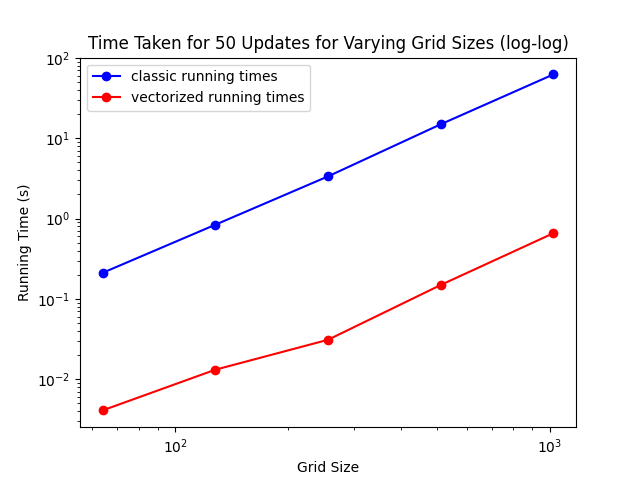
\includegraphics[width=\textwidth]{images/sub_v_vec_conway.png}
  \caption{Log-Log Plot of Running Times for the 2 Implemenations (varying grid sizes)}
  \label{fig:conway_docs}
\end{figure}

In the textual format, these were the running times that were visualized in the plot above:

\begin{lstlisting}[language=bash,basicstyle=\scriptsize\ttfamily]
$ python3 conway_profile.py
PROFILING COMPUTATION FOR classic_update (iters=50, runs=10)
Avg Time for 64x64: 0.21079003758495674
Avg Time for 128x128: 0.8369292417657561
Avg Time for 256x256: 3.3476251667947508
Avg Time for 512x512: 14.907938629109413
Avg Time for 1024x1024: 62.25631875410909
PROFILING COMPUTATION FOR numpy_vectorized_update (iters=50, runs=10)
Avg Time for 64x64: 0.004091558279469609
Avg Time for 128x128: 0.013126020890194923
Avg Time for 256x256: 0.03096429561264813
Avg Time for 512x512: 0.14896825831383467
Avg Time for 1024x1024: 0.657253283006139
\end{lstlisting}

It is clear to see speed-ups of up-to 100x with the help of the optimizations implemented. For smaller grid sizes (upto 128), the speed seems to be a little smaller. In the future, one could try to use the threshold approach described above to switch from \textit{separate} to \textit{in-place} arithmetic. 

In addition, below are the results of the \verb|line_profiler| when called on \verb|update_vectorized| method (a single run of 50 updates to a $64 \times 64$ grid): 

\begin{lstlisting}[language=bash,basicstyle=\tiny\ttfamily]
$% python3 -m line_profiler -rmt "conway_profile.py.lprof"
Timer unit: 1e-06 s

Total time: 0.012529 s
File: conway_profile.py
Function: update_vectorized at line 66

Line #      Hits         Time  Per Hit   % Time  Line Contents
==============================================================
    66                                           @profile                                                                   
    67                                           def update_vectorized(grid, n):                                            
    68                                               "The vectorized version of the grid update in conway's game of life"   
    69        50         69.0      1.4      0.6      intermediate_grid = np.zeros(grid.shape)                               
    70                                                                                                                      
    71                                               # Take the sum of the 8 neighbours, using in place operations          
    72        50       1320.0     26.4     10.5      intermediate_grid += np.roll(grid, (0, 1), (0, 1))                     
    73        50       1232.0     24.6      9.8      intermediate_grid += np.roll(grid, (0, -1), (0, 1))                    
    74        50       1192.0     23.8      9.5      intermediate_grid += np.roll(grid, (1, 0), (0, 1))                     
    75        50       1154.0     23.1      9.2      intermediate_grid += np.roll(grid, (-1, 0), (0, 1))                    
    76        50       1467.0     29.3     11.7      intermediate_grid += np.roll(grid, (1, 1), (0, 1))                     
    77        50       1440.0     28.8     11.5      intermediate_grid += np.roll(grid, (1, -1), (0, 1))                    
    78        50       1422.0     28.4     11.3      intermediate_grid += np.roll(grid, (-1, 1), (0, 1))                    
    79        50       1407.0     28.1     11.2      intermediate_grid += np.roll(grid, (-1, -1), (0, 1))                   
    80        50        205.0      4.1      1.6      intermediate_grid /= 255                                               
    81                                                                                                                      
    82        50        336.0      6.7      2.7      birth = (grid==OFF) & (intermediate_grid==3)                           
    83        50        524.0     10.5      4.2      die =  (grid==ON) & ((intermediate_grid < 2) | (intermediate_grid > 3))
    84        50        389.0      7.8      3.1      grid[birth] = ON                                                       
    85        50        372.0      7.4      3.0      grid[die] = OFF                                                        


Total time: 0.013271 s
File: conway_profile.py
Function: profile_vanilla_computation at line 94

Line #      Hits         Time  Per Hit   % Time  Line Contents
==============================================================
    94                                           @profile                                                                                        
    95                                           def profile_vanilla_computation(update_method_key):                                             
    96                                               # grid sizes increase by powers of 2                                                        
    97                                               # grid_sizes = [64, 128, 256, 512, 1024]                                                    
    98         1          1.0      1.0      0.0      grid_sizes = [64]                                                                           
    99                                               # times for each of the computations (in seconds)                                           
   100         1          0.0      0.0      0.0      times = []                                                                                  
   101                                               # number of iterations for which the updates will happen                                    
   102         1          1.0      1.0      0.0      max_iters = 50                                                                              
   103                                               # The number of times the run will be performed for each grid size.                         
   104                                               # The final running time reported will be the average of these runs                         
   105         1          0.0      0.0      0.0      num_runs = 1                                                                                
   106                                                                                                                                           
   107         1         21.0     21.0      0.2      print(...omitted for space...)
   108                                                                                                                                           
   109         2          0.0      0.0      0.0      for curr_size in grid_sizes:                                                                
   110         1          0.0      0.0      0.0          total_time = 0                                                                          
   111                                                                                                                                           
   112         2          0.0      0.0      0.0          for _ in range(num_runs):                                                               
   113         1        220.0    220.0      1.7              curr_grid = random_grid(curr_size)                                                  
   114                                                                                                                                           
   115         1          0.0      0.0      0.0              t1 = timer()                                                                        
   116        51         12.0      0.2      0.1              for _ in range(max_iters):                                                          
   117        50      13001.0    260.0     98.0                  UPDATE_DICT[update_method_key](curr_grid, curr_size)                            
   118         1          0.0      0.0      0.0              t2 = timer()                                                                        
   119                                                                                                                                           
   120         1          2.0      2.0      0.0              total_time += (t2 - t1)                                                             
   121                                                                                                                                           
   122         1          1.0      1.0      0.0          times.append(total_time / num_runs)                                                     
   123         1         11.0     11.0      0.1          print(...omitted for space...)                 
   124                                                                                                                                           
   125         1          1.0      1.0      0.0      return (grid_sizes, times)                                                                  


  0.01 seconds - conway_profile.py:66 - update_vectorized
  0.01 seconds - conway_profile.py:94 - profile_vanilla_computation
  \end{lstlisting}
  We can clearly see the significant reduction in the \verb|Per Hit| column for this vectorized profile (around 260 timer units) as opposed to the suboptimal, default profile mentioned in the \hyperref[sec:b3]{Profiling Existing Code} section above (around 30k timer units). When comparing the profile of the \verb|update_vectorized| function with that of the \verb|update| function from \hyperref[sec:b3]{Section 4.3}, we see that even though the \verb|Per Hit| cost of the lines inside the nested-loops of \verb|update| is low, these lines seem to be called a large number of times, causing the total time spent calling each of these lines to sky-rocket. This is in contrast to the \verb|update_vectorized| function -- where each line is invoked exactly 50 times, and even though the \verb|Per Hit| cost is high, the total cost is thus significantly lower. 

Finally, for a more visual proof of the speedup with the help of the vectorized methods can be found in the video in the working directory at \href{}{this} location. Here, we run the original \verb|conway.py| file (with visualization enabled) and a \verb|conway_improved.py| file -- which is the same file as \verb|conway.py| but which uses the vectorized method to perform grid-updates. Both these files perform updates to a $512 \times 512$ grid. In the video, it is evident how slow the normal \verb|update| method is compared to the vectorized and optimized \verb|update_vectorized| method. \\
\textit{Note: The grids might be different in the 2 implementations, since a seed was not used when initializing. Never-the-less, the clear visual difference in the speed of the updates to the grid remains evident.}
\section{Appendix}

% content end
%###############################################################################

% TODO: bibliograpghy when needed
% \printbibliography

\end{document}